\section{Background}
\label{sec:background}

We begin with an overview of essential concepts used in our work. After introducing the core ideas and terminology of the GORE methodology, including a tour of a sample goal model, we briefly introduce preference modeling and reasoning using CI-nets and their induced preference graphs (IPGs). 

\subsection{Goal-Oriented Requirements Engineering}
\label{sec:gore}

\begin{figure}%
\centering
\includegraphics[width=\columnwidth]{./figs/gore-cropped.pdf}%
\caption{Sample GORE goal model for online retailer}%
\label{fig:goal-model}%
\end{figure}

In GORE, requirements for a given system are represented as a \emph{goal model}, which illustrates the AND-OR decomposition of a \emph{root goal} into lower-level goals for the system. The root goal expresses the overall requirement for the system, while the lower-level goals specify aspects of the root in greater detail, including possible alternatives for satisfying a higher-level requirement. Given a goal model for a proposed system, correct implementations of the proposed system can be identified by computing satisfiable assignments to the leaf nodes of the goal model~\cite{Mylopoulos:CAiSE04}. 

Optionally, the goal model may also contain a set of \emph{softgoals} or \emph{optional goals}, which are not part of the system's core requirement set but are desirable properties for the system to possess. Because softgoals and/or optional goals are linked to goals within the AND-OR graph of the goal model, two different implementations of the system may support or interfere with different sets of softgoals or optional goals, even though they both fulfill the core requirements for the system. If preferences over the possible combinations of softgoals or optional goals are known, then possible implementations of the system can be prioritized according to these preferences~\cite{Liaskos:RE10}. 

%it is possible to prioritize the possible implementations of the system according to these preferences~\cite{Liaskos:RE10}. 

%%% Following is adapted from Ganesh.
Consider a goal model for an online retailer (Figure~\ref{fig:goal-model}), where each core function may be realized in multiple ways. The unshaded node at the root of the AND-OR tree represents the required overall functionality of the system: in this case, the system's main purpose is to allow users to buy books. The rest of the unshaded nodes represent sub-goals, which specify parts of the functionality needed to accomplish a higher-level goal (AND-decomposition) or alternative methods for fulfilling a higher-level goal (OR-decomposition). The shaded nodes represent non-functional properties (NFPs) that the system could possess, while the MAKE (green) edges and BREAK (red) edges indicate whether a sub-goal contributes to the satisfaction of an NFP or violates it, respectively. Observe that
there are many correct designs, which differ in terms of their NFPs: security ($S$), transaction
 costs ($C$) and traceability ($T$). 

%%% Following comes directly from Ganesh, including the figure.
Let the manager and the software architect be the two major stakeholders 
who influence the design decisions in the project. Suppose that the
manager holds preference P1, ``Cost is more important than Traceability, 
provided the design is Secure''. Further, suppose the architect holds 
preference P2, ``Traceability is more important than Security''. Any
design satisfying all three NFPs is trivially the most preferred design
that is consistent with the preferences of both the manager and the
architect. However, such a design is not realizable because all three
NFPs cannot be simultaneously optimized. 

The next best alternative would be a design that satisfies 
two of the NFPs. Among the pairs of NFPs, we can infer that $(T,C)$ is preferred to $(S,C)$ because of
the architect's preference (P2), and $(S,C)$ is preferred to $(S,T)$ because of the manager's preference (P1).
Because the goal model indicates that no correct design exists that satisfies $(T,C)$, we next explore the existence
of a correct design that satisfies $(S,C)$. Such a design exists, according to the goal model; moreover, it is provably the
most preferred correct design with respect to the preferences of the architect and manager.

\begin{figure}%
\centering
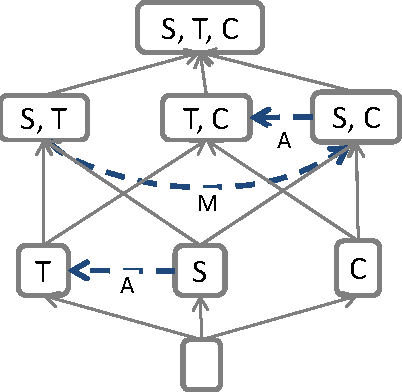
\includegraphics[width=0.5\columnwidth]{./figs/ipg-multi-stakeholder-noconflict-cropped.pdf}%
\caption{Induced preference graph for CI-net with preferences P1 and P2}%
\label{fig:ipg-no-conflict}%
\end{figure}

Although it is easy to identify the most preferred correct design manually for this small example, this
task becomes far more complicated in the presence of a large number of stakeholders and goal models
with many nodes. Moreover, there may arise conflicts among the preferences of the various stakeholders: 
for example, the manager may specify that Cost is more important than Traceability and Security, but
the architect may specify that Security is more important than Traceability and Cost. What is the most
preferred combination of NFPs to be satisfied in this case? How would the solution change if the manager's 
preferences take precedence over the architect's preferences due to the manager's higher authority?


\subsection{Conditional Importance Networks (CI-Nets)}
\label{sec:cinet}

%(\textbf{NOTE: the following brief overview of CI-nets is taken almost directly from my dissertation. 
%TODO revise and shorten this overview; also, make it consistent (w.r.t. notation) with the quick
%examples given in the intro section. For this audience, simpler is better.})
%
\emph{Conditional importance networks}
(CI-nets)~\cite{Bouveret:IJCAI2009} provide a formalized way to 
specify relative importance among sets of items. 
We will limit ourselves here to a high-level overview of CI-nets and
how they can be used; those who are interested in the details of 
CI-net semantics should consult~\cite{Bouveret:IJCAI2009} 
or~\cite{Santhanam:AAAI2010}. 

Suppose a group of system stakeholders is asked to decide which of
several non-functional properties are most important for a system to
provide; let $V$ be the set of all properties being considered. A
CI-net $\cinet$ is a set of preference statements, where each
statement contains four sets of items selected from $V$ that are 
%disjoint (i.e., no item appears in more than one set) and are
arranged as follows: 
\begin{quote}
\{\emph{true-conditions}\}, \{\emph{false-conditions}\} : \\
\{\emph{more-preferred-items}\} $\pref$ \{\emph{less-preferred-items}\}
\end{quote}
All four sets must be \emph{disjoint}, i.e., no two sets may
contain the same item. The \emph{true-conditions} and
\emph{false-conditions} sets may be empty, but \emph{more-preferred-items}
and \emph{less-preferred-items} must contain at least one
element. Informally, a CI-net statement means: 
``Given two sets of items, if all of the \emph{true-conditions}
are included in both sets and none of the \emph{false-conditions} are
included in either set, then the set that includes all of the
\emph{more-preferred-items} is preferred to the set that includes all
of the \emph{less-preferred-items}, all else being equal.'' 

Automated preference reasoning over a CI-net is possible because every
CI-net induces a strict partial order over the set of all possible
combinations of properties in $V$ (i.e., the powerset of $V$). 
This partial order is defined by combining the \emph{importance rules}
specified by the CI-net statements with a \emph{monotonicity rule}, 
which provides an intuitive default preference in the absence of
specific guidance. Informally, the monotonicity rule states that for
any two sets of items $A$ and $B$, if $B$ contains every item in $A$ 
plus at least one additional item (i.e., if $B \supset A$), then $B$ 
must be preferred to $A$ ($B \pref A$). As an example of the intuition
behind the monotonicity rule, if offered a choice between a new car
with minimal fuel included or the same new car with a full tank of
fuel (at the same price), most people would choose the car with more
fuel included. 
 
Using the CI-net's preference statements and the monotonicity rule, it
is possible to construct a graph where each node represents a different
set of properties selected from $V$ and each directed edge from one node
to another indicates that the set of properties at the destination node
is preferred to the set of properties at the source node. Such a graph
is referred to as the CI-net's \emph{induced preference graph} 
(IPG)~\cite{Bouveret:IJCAI2009}. An algorithm for constructing the
IPG of a CI-net is described in~\cite{Oster:FACS12}. 
Figure~\ref{fig:ipg-no-conflict} shows the IPG for the example 
preferences given in Section~\ref{sec:gore}, which can be expressed by
the following CI-net statements:
\begin{quote}
\begin{enumerate}
	\item[(P1)] $\{S\}, \{\} : \{C\}, \{T\}$
	\item[(P2)] $\{\}, \{\} : \{T\}, \{S\}$
	%\item[(P3)] $\{\}, \{\} : \{S\}, \{C\}$
\end{enumerate}
\end{quote}
%\begin{definition}[Induced Preference Graph]
%\label{def:induced-pref-graph}
%Given a CI-net $\cinet$ over a set of variables $V$, the \emph{induced
  %preference graph (IPG)} $\delta(\cinet) = (N, E)$ is constructed as
%follows. The nodes $N$ correspond to the powerset of $V$, and each
%directed edge $(\gamma, \gamma') \in E$ corresponds to an improving
%(monotonicity or importance) flip from $\gamma$ to $\gamma'$ as per
%the CI-net semantics (Definition~\ref{def:ci-flip}) such that
%$\gamma'\pref\gamma$.
%\end{definition}
%
%\begin{figure*}[!t]%
%\centering
%\includegraphics[width=0.7\textwidth]{./figs/applications-figure.pdf}%
%\caption{Four applications of our iPref-R preference reasoning framework, which is based on the use of CI-nets}%
%\label{fig:cinet-apps}%
%\end{figure*}

We discuss in Section~\ref{sec:pref-alt} our prior work toward integrating CI-nets into the context of the GORE framework, as well as our ongoing extensions of that work. In addition, we have applied CI-nets to model, analyze, and reason with preferences in a range of other problem domains, including:
%. Figure~\ref{fig:cinet-apps} illustrates the range of other problems that we have addressed using CI-nets, including:
\begin{enumerate}
	\item \emph{Trust negotiation}~\cite{Oster:FACS12}: Given several sets of credentials that can be used to authenticate a client to a server, what is the least sensitive set of credentials (with respect to the client's privacy preferences) that is sufficient to convince the server to grant access to the client? 
	%\item \emph{Goal-oriented requirements engineering}~\cite{Oster:ASE11}: Given a goal model annotated with a set of optional goals and MAKE/BREAK links between required and optional goals, which set of required goals completely fulfills the root goal in the goal model while also fulfilling the most preferred possible set of optional goals?
	%\item \emph{Embedded system design}~\cite{?}: Given several possible features and/or properties of a proposed embedded system, which possible feature set or configuration for the system is most preferred by the system's customers and/or end users? (cut because no citation available)
	\item \emph{Cybersecurity}~\cite{Santhanam:CSIIRW2013}: How can a computer system administrator select the best set of countermeasures to deploy in response to an attack on the system to most effectively thwart the attacker's expected goals while causing minimal disruption to authorized users?
	\item \emph{Sustainable building design}~\cite{Santhanam:AAAISpring11}: Given the tradeoffs between the costs and benefits of sustainable building features or practices in a construction project, which collection of features and/or practices will satisfy the sustainability preferences of the client at the lowest cost?
\end{enumerate}
